%!TEX root = main.tex

\section{Notes on category theoretic probability and string diagrams}

Category theoretic treatments of probability theory often start with \emph{probability monads} (for a good overview, see \citep{jacobs_probability_2018}). A monad on some category $C$ is a functor $T:C\to C$ along with natural transformations called the unit $\eta:1_C\to T$ and multiplication $\mu:T^2\to T$. Roughly, functors are maps between categories that preserve identity and composition structure and natural transformations are "maps" between functors that also preserve composition structure. The monad unit is similar to the identity element of a monoid in that application of the identity followed by multiplication yields the identity transformation. The multiplication transformation is also (roughly speaking) associative.

An example of a probability monad is the discrete probability monad given by the functor $\mathcal{D}:\textbf{Set}\to\textbf{Set}$ which maps a countable set $X$ to the set of functions from $X\to [0,1]$ that are probability measures on $X$, denoted $\mathcal{D}(X)$. $\mathcal{D}$ maps a measurable function $f$ to $\mathcal{D}f:X\to \mathcal{D}(X)$ given by $\mathcal{D}f:x\mapsto \delta_{f(x)}$. The unit of this monad is the map $\eta_X:X\to \mathcal{D}(X)$ given by $\eta_X:x\mapsto \delta_x$ (which is equivalent to $\mathcal{D} 1_X$) and multiplication is $\mu_X:\mathcal{D}^2(X)\to \mathcal{D}(X)$ where $\mu_X:\Omega\mapsto \sum_{\phi} \Omega(\phi) \phi$.

For continuous distributions we have the Giry monad on the category $\textbf{Meas}$ of mesurable spaces given by the functor $\mathcal{G}$ which maps a measurable space $X$ to the set of probability measures on $X$, denoted $\mathcal{G}(X)$. Other elements of the monad (unit, multiplication and map between morphisms) are the ``continuous'' version of the above.

Of particular interest is the Kleisli category of the monads above. The Kleisli $C_T$ category of a monad $T$ on category $C$ is the category with the same objects and the morphisms $X\to Y$ in $C_T$ is the set of morphisms $X\to TY$ in $C$. Thus the morphisms $X\to Y$ in the Kleisli category $\textbf{Set}_{\mathcal{D}}$ are morphisms $X\to \mathcal{D}(Y)$ in $\textbf{Set}$, i.e. stochastic matrices, and in the Kleisli category $\textbf{Meas}_{\mathcal{G}}$ we have Markov kernels. Composition of arrows in the Kleisli categories correspond to Matrix products and ``kernel products'' respectively.

Both $\mathcal{D}$ and $\mathcal{G}$ are known to be \emph{commutative} monads, and the Kleisli category of a commutative monad is a symmetric monoidal category.

Diagrams for symmetric monoidal categories consist of wires with arrows, boxes and a couple of special symbols. The identity object (which we identify with the set $\{*\}$) is drawn as nothing at all  $\{*\}:=\boxed{\hspace{2em}}$ and identity maps are drawn as bare wires:

\begin{align}
	\mathrm{Id}_X:=\begin{tikzpicture}[->]
	\path (0,0) node (A) {\hspace{1em}$X$}
	++(0,0.5) coordinate (B); 
	\draw (A.center) -- (B);
	\end{tikzpicture}
\end{align}

We draw Kleisli arrows from the unit (i.e. probability distributions) $\mu:\{*\}\to X$ as triangles and Kleisli arrows $\kappa:X\to Y$ (i.e. Markov kernels $X\to \Delta(\mathcal{Y})$) as boxes. We draw the Kleisli arrow $\mathds{1}_{X}:X\to\{*\}$ (which is unique for each $X$) as below
\begin{align}
	\mu:=
	\begin{tikzpicture}[->]
		\path (0,0) node[dist] (A) {$\mu$}
		++(0,0.5) node (B) {\hspace{2em}$X$};
		\draw (A)--(B.center);
	\end{tikzpicture}
	\hspace{2cm} \kappa:=
	\begin{tikzpicture}[->]
		\path (0,0) node[kernel] (A) {$\kappa$}
		++(0,0.5) node(B) {\hspace{2em}$Y$};
		\draw (A)--(B.center);
	\end{tikzpicture}
\end{align}

The product of objects in \textbf{Meas} is given by $(X,\mathcal{X})\cdot(Y,\mathcal{Y})=(X\times Y,\mathcal{X}\otimes\mathcal{Y})$, which we will often write as just $X\times Y$. Horizontal juxtaposition of wires indicates this product, and horizontal juxtaposition also indicates the tensor product of Kleisli arrows. Let $\kappa_1:X\to W$ and $\kappa_2:Y\to Z$:
\begin{align}
 (X\times Y,\mathcal{X}\otimes\mathcal{Y}) :=
 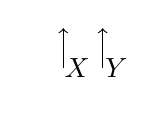
\begin{tikzpicture}[->]
	\path (0,0) node (A) {\hspace{1em}$X$}
	+(0,0.5) coordinate (B)
	++(0.5,0) node (C) {\hspace{1em}$Y$}
	+(0,0.5) coordinate (D); 
	\draw (A.center) -- (B);
	\draw (C.center) -- (D);
 \end{tikzpicture}
 \hspace{2cm} \kappa_1\otimes \kappa_2:=
 \begin{tikzpicture}
	\path (0,0) node (A) {\hspace{1em}$X$}
	+(0,0.5) node[kernel] (B) {$\kappa_1$}
	+(0,1) node (C) {\hspace{1em}$W$}
	++(0.8,0) node (D) {\hspace{1em}$Y$}
	+(0,0.5) node[kernel] (E) {$\kappa_2$}
	+(0,1) node (F) {\hspace{1em}$Z$}; 
	\draw (A.center) -- (B);
	\draw[->] (B) -- (C.center);
	\draw (D.center) --(E);
	\draw[->] (E) -- (F.center);
 \end{tikzpicture}
\end{align}

Composition of arrows is achieved by ``wiring'' boxes together. For $\kappa_1:X\to Y$ and $\kappa_2:Y\to Z$ we have


\begin{align}
\kappa_1\kappa_2(x;A)=\int_Y \kappa_2(y;A) \kappa_1(x;dy):=\begin{tikzpicture}
	\path (0,0) node (C) {\hspace{1em}$X$}
	++(0,0.5) node[kernel] (A) {$\kappa_1$}
	++(0,0.75) node[kernel] (B) {$\kappa_2$}
	++(0,0.5) node (D) {\hspace{1em}$Z$};
	\draw (C.center) -- (A);
	\draw (A) -- (B);
	\draw[->] (B) -- (D.center);
\end{tikzpicture}
\end{align}


Symmetric monoidal categoris have the following coherence theorem\citep{selinger_survey_2010}:

\begin{theorem}[Coherence (symmetric monoidal)]
	A well-formed equation between morphisms in the language of symmetric monoidal categories follows from the axioms of symmetric monoidal categories ifand only if it holds, up to isomorphism of diagrams, in the graphical language.
\end{theorem}

Isomorphism of diagrams for symmetric monoidal categories (somewhat informally) is any planar deformation of a diagram including deformations that cause wires to cross. We consider a diagram for a symmetric monoidal category to be well formed only if all wires point upwards.


In fact the Kleisli categories of the probability monads above have (for each object) unique \emph{copy}: $X\to X\times X$ and \emph{erase}: $X\to\{*\}$ maps that satisfy the \emph{commutative comonoid axioms} that (thanks to the coherence theorem above) can be stated graphically. These differ from the copy and erase maps of \emph{finite product} or \emph{cartesian} categories in that they do not necessarily respect composition of arrows.


\begin{align}
	\text{Erase} = \mathds{1}_X := 
	\begin{tikzpicture}
	    \path (0,0) coordinate (A)
	    ++ (0,0.5) node(B) {\textbf{*}};
	    \draw (A) -- (B.center);
	\end{tikzpicture}
	\text{Copy} = x\mapsto \delta_{x,x} := 
	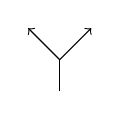
\begin{tikzpicture}[scale=0.8]
	\path (0,0) coordinate (A) 
	++ (0,0.5) coordinate (B)
	+ (0.5,0.5) coordinate (C)
	+ (-0.5,0.5) coordinate (D);
	\draw (A) -- (B);
	\draw[->] (B) -- (C);
	\draw[->] (B) -- (D);
	\end{tikzpicture}
\end{align}

\begin{align}
	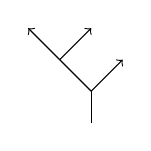
\begin{tikzpicture}[scale=0.8]
	\path (0,0) coordinate (A) 
	++ (0,0.5) coordinate (B)
	+ (0.5,0.5) coordinate (C)
	++ (-0.5,0.5) coordinate (D)
	+(0.5,0.5) coordinate (E)
	+(-0.5,0.5) coordinate (F);
	\draw (A) -- (B);
	\draw[->] (B) -- (C);
	\draw (B) -- (D);
	\draw[->] (D) -- (E);
	\draw[->] (D) -- (F);
	\end{tikzpicture}
	=
	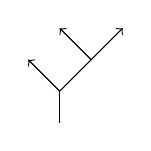
\begin{tikzpicture}[scale=0.8]
	\path (0,0) coordinate (A) 
	++ (0,0.5) coordinate (B)
	+ (-0.5,0.5) coordinate (C)
	++ (0.5,0.5) coordinate (D)
	+(0.5,0.5) coordinate (E)
	+(-0.5,0.5) coordinate (F);
	\draw (A) -- (B);
	\draw[->] (B) -- (C);
	\draw (B) -- (D);
	\draw[->] (D) -- (E);
	\draw[->] (D) -- (F);
	\end{tikzpicture}
	:=
		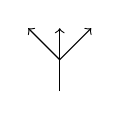
\begin{tikzpicture}[scale=0.8]
	\path (0,0) coordinate (A) 
	++ (0,0.5) coordinate (B)
	+ (-0.5,0.5) coordinate (C)
	+ (0,0.5) coordinate (D)
	+(0.5,0.5) coordinate (E);
	\draw (A) -- (B);
	\draw[->] (B) -- (C);
	\draw[->] (B) -- (D);
	\draw[->] (B) -- (E);
	\end{tikzpicture}\label{eq:ccom1}
\end{align}

\begin{align}
	\begin{tikzpicture}[scale=0.8]
	\path (0,0) coordinate (A) 
	++ (0,0.5) coordinate (B)
	+ (0.5,0.5) coordinate (C)
	+ (-0.5,0.5) node (D) {\textbf{*}};
	\draw (A) -- (B);
	\draw[->] (B) -- (C);
	\draw (B) -- (D.center);
	\end{tikzpicture}
	= 
	\begin{tikzpicture}[scale=0.8]
	\path (0,0) coordinate (A) 
	++ (0,0.5) coordinate (B)
	+ (0.5,0.5) node (C) {\textbf{*}}
	+ (-0.5,0.5) coordinate (D) ;
	\draw (A) -- (B);
	\draw (B) -- (C.center);
	\draw[->] (B) -- (D);
	\end{tikzpicture}
	=
	\begin{tikzpicture}[scale=0.8]
	\path (0,0) coordinate (A) 
	++ (0,1) coordinate (B);
	\draw[->] (A) -- (B);
	\end{tikzpicture}\label{eq:ccom2}
\end{align}

\begin{align}
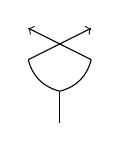
\begin{tikzpicture}[scale=0.8]
	\path (0,0) coordinate (A) 
	++ (0,0.5) coordinate (B)
	+ (0.5,0.5) coordinate (C)
	+ (-0.5,0.5) coordinate (D)
	+(0.5,1) coordinate (E)
	+(-0.5,1) coordinate (F);
	\draw (A) -- (B);
	\draw (B) to [bend right] (C);
	\draw (B) to [bend left] (D);
	\draw[->] (C) to  (F);
	\draw[->] (D) to  (E);	
\end{tikzpicture}
=
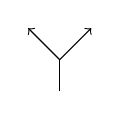
\begin{tikzpicture}[scale=0.8]
	\path (0,0) coordinate (A) 
	++ (0,0.5) coordinate (B)
	+ (0.5,0.5) coordinate (C)
	+ (-0.5,0.5) coordinate (D);
	\draw (A) -- (B);
	\draw[->] (B) -- (C);
	\draw[->] (B) -- (D);
\end{tikzpicture}\label{eq:ccom3}
\end{align}

Finally, $\{*\}$ is a terminal object in the Kleisli categories of either probability monad. This means that the map $X\to\{*\}$ is unique for all objects $X$, and as a consequence for all objects $X,Y$ and all $\kappa:X\to Y$ we have
\begin{align}
\begin{tikzpicture}
 \path (0,0) node (A) {\hspace{1em}$X$}
 ++(0,0.5) node[kernel] (B) {$\kappa$}
 ++(0,0.5) node (C) {\textbf{*}};
 \draw (A.center) -- (B);
 \draw (B) -- (C.center);
\end{tikzpicture}
=
\begin{tikzpicture}
 \path (0,0) node (A) {\hspace{1em}$X$}
  ++(0,0.5) node (C) {\textbf{*}};
 \draw (A.center) -- (C.center);
\end{tikzpicture}\label{eq:termobj}
\end{align}
This is equivalent to requiring for all $x\in X$ $\int_Y \kappa(x;dy)=1$. In the case of $\textbf{Set}_\mathcal{D}$, this condition is what differentiates a stochastic matrix from a general positive matrix (note that positive matrices live in a larger category than $\textbf{Set}_\mathcal{D}$). In the case of $\textbf{Meas}_\mathcal{G}$, Markov kernels require an additional measurability condition for which I am not presently aware of any graphical statement.

Thus when manipulating diagrams representing Markov kernels in particular (and, importantly, not more general symmetric monoidal categories) diagram isomorphism also includes applications of \ref{eq:ccom1}, \ref{eq:ccom2}, \ref{eq:ccom3} and \ref{eq:termobj}.